%\newcommand{\tool}{NCGOP~}

\section{Evaluation}\label{sec:application}
\noindent\textbf{Implementation.} To conduct a fair comparison between the MOIP methods and other MOEAs, we use the existing EAs from the open source tool of IBED \cite{DBLP:journals/asc/XueZT0CC016}. We implement these MOIP methods in the \textsc{IBED} framework. These MOIP methods are mainly implemented in Java, only the IP solving method uses the APIs of \textsc{Cplex}~\cite{CPLEX}. Our tool and experimental data are published at~\cite{ourtool}.%\footnote{CPLEX: The industrial solution for IP. \url{https://www-01.ibm.com/software/commerce/optimization/cplex-optimizer/}}. Our tool and experimental data are published at [].\footnote{IBED's tool \cite{DBLP:journals/asc/XueZT0CC016} is open-source. It extends the implementation of feedback-directed IBEA \cite{DBLP:conf/issta/TanXCSLD15} that is based on the open-source library \textsc{jMetal}.}

\noindent\textbf{Research Questions.} For \naiveSol~and CWMOIP that search for all non-dominant solutions, we answer the RQ1-RQ2.
For \ourSol~that aims to efficiently find evenly-distributed non-dominant solutions, we compare it with the state-of-the-art MOEAs (i.e., IBED and IBEA) and answer the RQ3-RQ5:
%We conducted the experiments to evaluate the above approaches from different aspects.
\vspace{-1mm}
\begin{enumerate}[label=\textbf{RQ\arabic*.},itemindent=*,itemsep=0.1mm]
\item On small systems, can  the \naiveSol~and CWMOIP guarantee the \emph{completeness} of non-dominant solutions?
\item On small systems, what is the \emph{performance} of the \naiveSol~and CWMOIP?

\item On medium-to-large systems, can \ourSol~find \emph{abundant} and \emph{non-dominant} solutions?

\item On medium-to-large systems, can \ourSol~find \emph{evenly-distributed} non-dominant solutions ?

\item On large industrial systems, is  \ourSol~\emph{scalable}?

\end{enumerate}
\subsection{Setup}\label{subsection:qualityindicator}~\label{ssec:setup}
\vspace{-3mm}
\subsubsection{Baseline Tools}\label{subsecc:implementationsetup}
%We have implemented our approach based on \textsc{jMetal}~\cite{DBLP:journals/aes/DurilloN11}, which is a Java-based open source framework that supports multi-objective optimization with EAs.
Sayyad \emph{et.al} \cite{DBLP:conf/icse/SayyadMA13,conf/cmsbse/SayyadMA13} reported that IBEA implemented in \textsc{jMetal} shows best results for the optimal feature selection. %Later, Tan \emph{et.al} \cite{DBLP:conf/issta/TanXCSLD15} also proposed the feedback-directed mechanism to improve existing MOEAs. In these studies, IBEA is reported as the best MOEA for this problem.
Recently, according to \cite{DBLP:journals/asc/XueZT0CC016}, on most systems (except $eCos$), IBED finds more non-dominant solutions than IBEA in similar time.  IBEA and IBED represent the-state-of-art approaches and they are publicly available. Hence, we choose them as the baseline tools for comparison.

%\textbf{IBEA}: Indicator-Based Evolutionary Algorithm ~\cite{DBLP:conf/ppsn/ZitzlerK04}.

%\begin{enumerate}[itemindent=*,itemsep=0.1mm]
%   \item \textbf{our approach}: our Indicator-Based Differential Evolutionary
%   \item \textbf{IBEA}: Indicator-Based Evolutionary Algorithm ~\cite{DBLP:conf/ppsn/ZitzlerK04}
%  \item \textbf{NSGA-II}: Nondominated Sorting Genetic Algorithm ~\cite{DBLP:journals/tec/BradstreetWB08}
%  \item \textbf{ssNSGA-II}: Steady-state NSGA-II ~\cite{coello2004applications}
%  \item \textbf{MOCell}: A Cellular Genetic Algorithm for Multi-objective Optimization~\cite{miettinen1999nonlinear}
%\end{enumerate}
%A brief overview of these EAs are provided in~\mtable{table:EAOverview}.

% Table generated by Excel2LaTeX from sheet 'Sheet1'
% Table generated by Excel2LaTeX from sheet 'Sheet1'

\subsubsection{Baseline Tools Configurations}
We adopt the version of IBEA and IBED that produce the best results according to \cite{DBLP:conf/issta/TanXCSLD15}\cite{DBLP:journals/asc/XueZT0CC016} --- actually the same enhancement for them, namely \textbf{IBED $F+P$} and \textbf{IBEA $F+P$}. Here $F+P$ refers to the configuration that enables feedback-directed mechanism \cite{DBLP:conf/issta/TanXCSLD15} and preprocessing for core feature encoding \cite{DBLP:journals/tosem/HieronsLLSZ16}.
%\begin{enumerate}[label=\alph*),itemsep=0.1mm]
 % \item \textbf{IBEA $F+P$}: the IBEA version that enable feedback-directed mechanism \cite{DBLP:conf/issta/TanXCSLD15} and pre.
  %  \item \textbf{IBED $F+P$}: the IBED version that enable feedback-directed mechanism and core
%  \item \textbf{U+P}: The unguided version of EA with preprocessing  (\msection{ssec:preprocess}) applied before the execution of the unguided EA. We have demonstrated that, our method has found more prunable features than the preprocessing method of~\cite{DBLP:dblp_conf/kbse/SayyadIMA13} in~\msection{subsecc:featuremodelsetup}; therefore, U+P can be seen as an improved version of~\cite{DBLP:dblp_conf/kbse/SayyadIMA13} with smaller search space.
%  \item \textbf{U}: The unguided version of EA without preprocessing, which is used by~\cite{DBLP:conf/icse/SayyadMA13,conf/cmsbse/SayyadMA13}.

   %this is essentially the version that has been used in~\cite{DBLP:conf/icse/SayyadMA13}, which is the current state-of-the-art method to the knowledge of the authors.
%\end{enumerate}


%\begin{table}[t]
%  \centering
%  \vspace{-2mm}
%    \caption{Feature Models}
%   \scalebox{0.85}{
%   % Table generated by Excel2LaTeX from sheet 'Sheet2'
%\begin{tabular}{|>{\centering\arraybackslash}m{0.5cm}|>{\centering\arraybackslash}m{1.2cm}|>{\centering\arraybackslash}m{0.7cm}|>{\centering\arraybackslash}m{0.95cm}|>{\centering\arraybackslash}m{0.6cm}|>{\centering\arraybackslash}m{0.6cm}|>{\centering\arraybackslash}m{0.95cm}|}
%\hline
%\multicolumn{1}{|c|}{\textbf{Repo.}} & \textbf{Sys.} & \textbf{Fea.} & \textbf{Cons.} & \textbf{$F_p$} & \textbf{$F_p'$} & \multicolumn{1}{c|}{\textbf{Ref.}} \bigstrut\\
%\hline
%    --  & JCS   & 12    & 13    &    2   &    --  & -- \bigstrut\\
%\hline
%\multicolumn{1}{|c|}{\multirow{2}[4]{*}{SPLOT}} & Web Portal & 43    & 36    &    4   &    --   & \cite{DBLP:conf/sac/MendoncaBC08}
%  \bigstrut\\
%\cline{2-7}\multicolumn{1}{|c|}{} & E-Shop & 290   & 186   &   28    &   --    & \cite{DBLP:conf/wcre/XueXJ10} \bigstrut\\
%\hline
%\multicolumn{1}{|c|}{\multirow{4}[10]{*}{LVAT}} & eCos  & 1244  & 3146  &  54     &  19     & \cite{DBLP:conf/icse/SheLBWC11,DBLP:conf/wcre/XueXJ10} \bigstrut\\
%%\cline{2-7}\multicolumn{1}{|c|}{} & FreeBSD & 1396  & 62183 &    41   &    3  & \cite{DBLP:conf/icse/SheLBWC11,thTechnireport10} \bigstrut\\
%%\cline{2-7}\multicolumn{1}{|c|}{} & Fiasco & 1638  & 5228  &   1013    &   995   &\cite{Berger12variabilitymodeling}  \bigstrut\\
%\cline{2-7}\multicolumn{1}{|c|}{} & uClinux & 1850  & 2468  &   1244    &  1244    & \cite{Berger12variabilitymodeling} \bigstrut\\
%\cline{2-7}\multicolumn{1}{|c|}{} & Linux X86 & 6888  & 343944 &   156    &   94    & \cite{DBLP:conf/icse/SheLBWC11} \bigstrut\\ %,thTechnireport10
%\hline
%\end{tabular}%
%     }
%
%\vspace{-4mm}
%  \label{table:feaModel}%
%\end{table}%

% Table generated by Excel2LaTeX from sheet 'Sheet4'
% Table generated by Excel2LaTeX from sheet 'Sheet4'
\begin{table}[bp]
 
  \centering
  \scriptsize
    \caption{Feature Models used in experiments}
    \begin{tabular}{|c|c|c|c|c|}
    \hline
    \textbf{Repo.} & \textbf{Sys.} & \textbf{Fea.} & \textbf{Cons.} & \multicolumn{1}{c|}{\textbf{Ref.}} \bigstrut\\
    \hline
    \multirow{3}[6]{*}{SPLOT} & JCS   & 12    & 12    &  \cite{DBLP:conf/issta/TanXCSLD15} \bigstrut   \\
\cline{2-5}          & Web Portal & 43    & 36    &  \cite{DBLP:conf/sac/MendoncaBC08} \bigstrut\\
\cline{2-5}          & E-Shop & 290   & 186   &  \cite{DBLP:conf/wcre/XueXJ10} \bigstrut\\
    \hline
    \multirow{3}[6]{*}{LVAT} & eCos  & 1244  & 3146  &  \cite{DBLP:conf/icse/SheLBWC11,DBLP:conf/wcre/XueXJ10} \bigstrut\\
\cline{2-5}          & uClinux & 1850  & 2468  &  \cite{Berger12variabilitymodeling} \bigstrut\\
\cline{2-5}          & LinuxX86 & 6888  & 343944 & \cite{DBLP:conf/icse/SheLBWC11}  \bigstrut\\
    \hline
    \end{tabular}%
 
  \label{table:feaModel}%
\end{table}%



% Table generated by Excel2LaTeX from sheet 'Sheet3'

\begin{table*}[t]
  \centering
  \scriptsize
  \vspace{-3mm}
  \caption{Non-dominant solutions found by $\epsilon$-constraint (\textbf{A})  and CWMOIP  (\textbf{B})   on two small models, with 4 attribute sets for each model}
    \begin{tabular}{|c|c|c|c|c|c|c|c|c|c|c|c|c|c|c|}
   \Xhline{2\arrayrulewidth}
    System & A \%Corr & B \%Corr & A Time(s) & B Time(s) &A HV & B HV & A SP & B SP & $|A|$ & $|B|$ & $|A \cap B|$ & \textbf{$|N_A \cup N_B|$} & \textbf{$|N^{U}_A|$} & \textbf{$|N^{U}_B|$} \bigstrut\\
   \Xhline{2\arrayrulewidth}
    JCS 1 & 100   & 100   & 5.11  & 1.66  & 0.29  & 0.29  & 0.69  & 0.69  & 39    & 39    & 39    & 39    & 0     & 0 \bigstrut\\
    \hline
    JCS 2 & 100   & 100   & 6.84  & 0.67  & 0.27  & 0.27  & 0.39  & 0.39  & 9     & 9     & 9     & 9     & 0     & 0 \bigstrut\\
    \hline
    JCS 3 & 100   & 100   & 3.54  & 0.96  & 0.29  & 0.29  & 0.43  & 0.43  & 22    & 22    & 22    & 22    & 0     & 0 \bigstrut\\
    \hline
    JCS 4 & 100   & 100   & 7.92  & 1.97  & 0.25  & 0.25  & 0.56  & 0.56  & 31    & 31    & 31    & 31    & 0     & 0 \bigstrut\\
    \hline
    Web Portal 1 & 100   & 100   & 570.68  & 212.22  & 0.34  & 0.34  & 0.87  & 0.87  & 451   & 451   & 451   & 451   & 0     & 0 \bigstrut\\
    \hline
    Web Portal 2 & 100   & 100   & 692.88  & 256.38  & 0.31  & 0.31  & 0.98  & 0.98  & 768   & 768   & 768   & 768   & 0     & 0 \bigstrut\\
    \hline
    Web Portal 3 & 100   & 100   & 696.83  & 237.75  & 0.32  & 0.32  & 0.92  & 0.92  & 859   & 859   & 859   & 859   & 0     & 0 \bigstrut\\
    \hline
    Web Portal 4 & 100   & 100   & 564.82  & 163.97  & 0.33  & 0.33  & 0.96  & 0.96  & 713   & 713   & 713   & 713   & 0     & 0 \bigstrut\\
    \hline
    \end{tabular}%
  \label{tab:naiveVScwmoip}%
\vspace{-3mm}
\end{table*}%

\subsubsection{Parameter Settings}
 %For $U$, the same as~\cite{conf/cmsbse/SayyadMA13}, single-point crossover and bit-flip mutation are used as crossover and mutation operators, with crossover and mutation probabilities set to 0.1 and 0.01 respectively. These operators and probabilities also apply to $U+P$.
 For the $F+P$ version of EAs, %the feedback-directed  crossover  and feedback-directed mutation operators are used.
according to \cite{DBLP:conf/issta/TanXCSLD15}\cite{DBLP:journals/asc/XueZT0CC016},  the best setting of error mutation probability, mutation probability, and crossover probability are  1.0, 0.0000001, and 0.1 respectively. %Note in \mtable{table:lvat}, configuration $\mathit{F'+P}$ is the same as $\mathit{F+P}$, with the exception that the mutation probability $\mathit{P_{mut}}$ is set to 0.01.
%We run two settings for crossover probability $P_{cross}$, and mutation probability $P_{mut}$, which are $P_1=\{P_{Cross}=0.9, P_{mut}=0.05\}$ and $P_2=\{P_{Cross}=0.1, P_{mut}=0.01\}$. Configuration $U$ with parameter setting $P_1$ is used in ~\cite{DBLP:conf/icse/SayyadMA13}, and configuration $U$ with  parameter setting $P_2$ is used in ~\cite{conf/cmsbse/SayyadMA13}. These are the state-of-the-art methods for the optimal feature selection, to the knowledge of the authors.
For SPLOT systems in Table \ref{table:feaModel}, 25000 evaluations are used  for IBEA and IBED. For larger LVAT systems, 100000 evaluations are used for both EAs. For any model, we generate 10 sets of attributes. For each set, we run each EA repeatedly for 30 times and use their union to compare with \ourSol. Besides, the medium execution (the medium values of metrics) is compared with \ourSol~using 50 reference points. %The evaluation results for SPLOT and LVAT are reported in~\mtable{table:splot} and~\mtable{table:lvat}, respectively.
All other parameter settings for EAs are default settings of \textsc{jMetal} (e.g., population size is set to 100) are same as those used in \cite{DBLP:conf/icse/SayyadMA13}\cite{conf/cmsbse/SayyadMA13}\cite{DBLP:conf/issta/TanXCSLD15}\cite{DBLP:journals/asc/XueZT0CC016}.

In MOIP methods,  one common parameter is needed --- time limited for function $bintprog$. We set it as 0.1s for all system except for \emph{Linux X86} (10s for this system due to its huge number of constraints). The setting for reference point number in \ourSol~is 1000 for SPLOT  systems and 1500 for LVAT.


 The experiments were performed on an Intel Core I7 4710HQ CPU with 8 GB RAM, running on Windows 8.1.
%
%\paratitle{Parameters Setup} The mutation and crossover rates for rGA are set to 0.01% and 0.9%
%respectively. In addition, the population size is set to 20, the number
%of generations is set to 20.

\subsubsection{Quality Indicators}

To measure the quality of Pareto front, we adopt four indicators in this work:  percentage of correctness, hypervolume~\cite{DBLP:journals/tec/ZitzlerT991}, spread~\cite{DBLP:journals/tec/BradstreetWB08} and Pareto dominance.

%Hypervolume~\cite{DBLP:journals/tec/ZitzlerT991} is a measure measures of the volume of the dominated portion of the objective space.
% \begin{figure}[t]
%\centering
%\includegraphics[width=2.5in]{image/space}
%\caption{Hypervolume of a solution set with three solutions}
%\label{fig:hyper}
%\end{figure}

\begin{enumerate}[label=\alph*), itemsep=0.1mm]

  \item \textbf{\emph{Percentage of Correctness} (\%Cor)}:  For MOEAs, not all solutions are correct, as correctness is an objective evolving over time. Thus, for a solution set, the percentage of correct solutions inside indicates its quality.
  \item \textbf{\emph{Hypervolume (HV)}}: Hypervolume of the solution set $S$ is the volume of the region that is dominated by $S$ in the objective space. In \textsc{jMetal}, %though all objectives are minimized, the Pareto front is inverted before HV is calculated. Thus,
      the Pareto front with a higher HV is preferred.


\item \textbf{\emph{Spread (SP)}}: Spread is  used to measure the extend of spread in the obtained solutions.% and it is calculated using the following equation:
%\vspace{-1mm}
%\begin{equation}\label{eq:spread}
%\scriptsize
%Spread= \frac{d_f+d_l+\sum_{i=1}^{N-1}|d_i-\bar{d}|}{d_f+d_l+(N-1)\bar{d}}
%\end{equation}

\item \textbf{\emph{Num. of Pareto non-dominance}}: On the same set of feature attribute values, we can approximate the true Pareto front by the union of the two sets of solutions. On this Pareto front, we count the non-dominant solutions.
 %The larger the num. is, the higher quality the solutions are of. }
%      where $\mathit{N}$ is the number of points in the Pareto front, $\mathit{d_i}$ is Euclidean distances between consecutive points,  $\mathit{\bar{d}}$ is the average of $\mathit{d_i}$, $\mathit{d_f}$ and $\mathit{d_l}$ are the Euclidean distances between the extreme solutions and boundary solutions of the Pareto front respectively.
\end{enumerate}


%Other quality indicators, e.g., generational distance, inverted generational distance, epsilon and generalized speed, are used elsewhere. These indicators are not adopted in this experiment since they are used to compare the calculated Pareto front with the actual true Pareto front, which we do not have in this case.



% Table generated by Excel2LaTeX from sheet 'formated results'
\begin{table*}[t]
  \centering
   \scriptsize
   \vspace{-1mm}
  \caption{Non-dominant solutions found by CWMOIP (\textbf{A}) and  IBED $F+P$ (\textbf{B}) on two small models, with 4 attribute sets for each model}
    \begin{tabular}{|c|c|c|c|c|c|c|c|c|c|c|c|c|c|c|}
  \Xhline{2\arrayrulewidth}
    System & A \%Corr & B \%Corr & A Time(s) & B Time(s) &A HV & B HV & A SP & B SP & $|A|$ & $|B|$ & $|A \cap B|$ & \textbf{$|N_A \cup N_B|$} & \textbf{$|N^{U}_A|$} & \textbf{$|N^{U}_B|$} \bigstrut\\
   \Xhline{2\arrayrulewidth}
    JCS 1 & 100   & 92.37  & 1.66  & 150.66  & 0.29  & 0.28  & 0.69  & 0.28  & 39    & 19    & 19    & 39    & 20    & 0 \bigstrut\\
    \hline
    JCS 2 & 100   & 91.72  & 0.67  & 131.19  & 0.27  & 0.27  & 0.39  & 0.39  & 9     & 9     & 9     & 9     & 0     & 0 \bigstrut\\
    \hline
    JCS 3 & 100   & 85.80  & 0.96  & 135.38  & 0.29  & 0.28  & 0.43  & 0.31  & 22    & 17    & 17    & 22    & 5     & 0 \bigstrut\\
    \hline
    JCS 4 & 100   & 84.77  & 1.97  & 135.20  & 0.25  & 0.24  & 0.56  & 0.54  & 31    & 20    & 20    & 31    & 11    & 0 \bigstrut\\
    \hline
    Web Portal 1 & 100   & 98.00  & 212.22  & 162.80  & 0.34  & 0.33  & 0.87  & 0.45  & 451   & 232   & 97    & 451   & 354   & 0 \bigstrut\\
    \hline
    Web Portal 2 & 100   & 98.73  & 256.38  & 166.67  & 0.31  & 0.30  & 0.98  & 0.63  & 768   & 277   & 116   & 768   & 652   & 0 \bigstrut\\
    \hline
    Web Portal 3 & 100   & 99.63  & 237.75  & 156.52  & 0.32  & 0.31  & 0.92  & 0.66  & 859   & 386   & 184   & 859   & 675   & 0 \bigstrut\\
    \hline
    Web Portal 4 & 100   & 96.93  & 163.97  & 163.69  & 0.33  & 0.32  & 0.96  & 0.73  & 713   & 327   & 167   & 713   & 546   & 0 \bigstrut\\
    \hline
    \end{tabular}%
  \label{tab:cwmoipVSibed}%
\vspace{-3mm}
\end{table*}%


\subsection{Evaluation Systems}\label{sec:cases}

\subsubsection{System Selection}\label{subsecc:featuremodelsetup}

Feature models of different systems are used in experiments. Table \ref{table:feaModel} shows  repository name (\emph{Repo.}),  the model's system name (\emph{Sys.}), number of features (\emph{Fea.}),  number of constraints (\emph{Cons.}), and relevant literatures (\emph{Ref.}).


Three models are from SPLOT, a repository used by many researchers as a benchmark \cite{DBLP:conf/oopsla/MendoncaBC091}. $\JCS$ model is the running example of the paper. %Two feature models \emph{Web Portal} and \emph{E-Shop} are from SPLOT respository~, which is a repository used by many researchers as a benchmark.
\emph{Web Portal} model captures the configurations of Web portal product line, and \emph{E-Shop} model %, as one of the largest feature models in SPLOT,
captures a B2C system with fixed priced products. %These two models are chosen to facilitate the comparison with~\cite{DBLP:conf/icse/SayyadMA13}.
%To further evaluate the scalability,
Industrial systems' models from the Linux Variability Analysis Tools (LVAT) repository~\cite{LVAT} are used. %The models in LVAT were reversed-engineered from industrial systems.
%In contrast with SPLOT,
LVAT's models (e.g., \emph{Linux X86}) have  much more features and constraints.
All these models are chosen to facilitate the comparison with~\cite{DBLP:conf/icse/SayyadMA13}\cite{DBLP:conf/issta/TanXCSLD15}\cite{DBLP:journals/asc/XueZT0CC016}.

%Note that $\mathit{F_p}$ always contains the same number or more features than $\mathit{F_p'}$ -- this shows that our preprocessing method  with~\malgo{algo:filter}  has found more prunable features than~\cite{DBLP:dblp_conf/kbse/SayyadIMA13}. In~\cite{DBLP:dblp_conf/kbse/SayyadIMA13}, their preprocessing method is based on static analysis. In particular, they detect  always true disjunctions (rules) with only one feature, which means the feature is either a common feature or a dead feature. In addition, they investigate the disjunctions (rules) that include two features, if one of them is prunable in the first round, and the other one could be prunable as well. It is easy to see that our method based on SAT solving could detect all features that could be found by preprocessing method in~\cite{DBLP:dblp_conf/kbse/SayyadIMA13}, and it can be shown that $\mathit{F_p}$ is always not fewer than $\mathit{F_p'}$.

\subsubsection{Feature Attribute}

Each feature in each model has the following attributes, which are identical to attributes used in~\cite{DBLP:conf/icse/SayyadMA13}:

\begin{enumerate}[label=\textbf{\arabic*.},itemindent=*,itemsep=0.1mm]
  \item \textbf{\emph{Cost}}  $\in \grandr$, records the price incurred to include the feature. For each feature, the \emph{Cost} value is assigned with a real number that is normally distributed between 5.0 and 15.0.
  \item \textbf{\emph{Used\_Before}} $\in \{true, false\}$, records whether this feature was used before --- \emph{true}  for \lq\lq{}yes\rq\rq{} and \emph{false} for \lq\lq{}no\rq\rq. \emph{Used\_Before} values are uniformly distributed for features.
%  \item \textbf{\emph{Defects}} $\in \grandZ$, records the number of defects known in the feature. For each feature, the \emph{Defects} value is assigned with a real number that is normally distributed between 5 and 15. However, if the feature has not been used before, the \emph{Defects} value is set to 0.
  \item \textbf{\emph{Defects}} $\in \grandZ$, records the number of defects in the feature. For each feature, the \emph{Defects} value is assigned with an integer value normally distributed between 0 and 10. %However, if the feature has not been used before, the \emph{Defects} value is set to 0.
\end{enumerate}


%These three attributes provides three optimization objectives, i.e., to minimize total cost, to maximize features that have been used and to minimize the total number of known defects.

%\subsubsection{Optimization Objectives}
%We introduce the five optimization objectives that we use in the experiment in the following.
%Note that since jMetal requires minimization of the objectives; all objectives listed here are objectives to be minimized.
%\begin{enumerate}[label=\textbf{Obj\arabic*.},itemindent=*,itemsep=0.1mm]
%  \item \emph{Correctness}: minimize the number of violated constraints of the feature model.
%  \item \emph{Richness of features:} minimize the number of features that are not selected.
%  \item \emph{Cost:} minimize the total cost.
%  \item \emph{Feature used before:} minimize the number of features that have not been used before.
%  \item \emph{Defects:} minimize the number of known defects.
%\end{enumerate}
%
%We specify correctness as an objective, rather than a constraint. The reason is that this allows EA to nudge the search towards feature models that contain fewer violated constraints, which eventually lead to valid feature models that do not contain violated constraints. Furthermore, note that some objectives are conflicting, e.g., Obj2 and Obj3, because the richness of features would imply a higher cost, but at the same time the cost needs to be minimized.

\subsection{Results}\label{sec:results}
To accurately compare the quality of solutions found by two methods, we check Pareto dominance-relation and other indicators (HV, SP and time).
In Table \ref{tab:naiveVScwmoip}, \ref{tab:cwmoipVSibed}, \ref{tab:ourSolVSibed} and \ref{tab:ourSolVSibea}, we  record the  \emph{\textbf{correct}} solutions  found by the first method in  column \textbf{$|A|$}, and those by the second one in column \textbf{$|B|$}. Column \textbf{$|A  \cap  B|$}  shows  the  number  of  \textbf{\emph{correct  solutions  commonly  found}}  by both methods. After non-dominance sorting, column  $|N_A \cup  N_B|$  lists  the  number of \emph{\textbf{the union of correct non-dominant}} solutions found  by  both  methods.  We also  list  the  number  of correct \emph{\textbf{unique non-dominant}} solutions  found  only by  the first  (or the second) method  in  column  $|N^U_A|$  (or  $|N^U_B|$).
To mitigate the bias due to one-time execution of EAs,  we compare MOIP methods with them based on the union of non-dominant solutions found by 30 executions of EAs.  $|Time(s)|$ refers to the total time ---- for EAs, it is total time for 30 executions. To get $|HV|$ and $|SP|$, we approximate true Pareto front with  $|N_A \cup  N_B|$ and use that as reference points.

We first evaluate the $\epsilon$-constraint and CWMOIP that aim to find all non-dominant solutions.

\subsubsection{RQ1---Solution Set Completeness on Small Systems}\label{sec:results:rq1}
As shown in  Table \ref{tab:naiveVScwmoip}, on 4 different sets of feature attributes of each model, we can always find \textbf{$|A|$}=\textbf{$|B|$}= $|N_A \cup  N_B|$, which means they found exactly same solutions. As the completeness of the $\epsilon$-constraint and CWMOIP has been proven in \cite{e-constraint}\cite{DBLP:journals/eor/OzlenA09}, we confirm this by the experiments.
Comparing CWMOIP with IBED  in  Table \ref{tab:cwmoipVSibed}, we see \textbf{IBED cannot find all non-dominant solutions with 30 executions in most cases} (except \emph{JCS2} that  has only 9 non-dominant solutions). In most cases, IBED's results are unsatisfactory, covering averagely about $70\%$ of the true Pareto front on 4 attribute sets of \emph{JCS}, and about $20\%$ of the true Pareto front on \emph{Web Portal}. Also,  we find $|N_A \cup  N_B|= |A|$, which proves the completeness of $|A|$.
% Table generated by Excel2LaTeX from sheet 'Sheet3'
\subsubsection{RQ2---Performance on Small Systems}\label{sec:results:rq2}
In Table \ref{tab:cwmoipVSibed}, we can see that it takes averagely about 5s for \naiveSol~method and 1.5s for CWMOIP on 4 attribute sets of \emph{JCS}, and averagely about 613s for \naiveSol~method and 218s for CWMOIP on 4 attribute sets of \emph{Web Portal}.
In contrast, one medium execution of IBED (i.e., the one with the medium size of $|A|$ in 30 executions)  on \emph{JCS 1} takes about 4.5s to find $17$ correct solutions. Actually, on \emph{JCS 1}, 30 executions just brings several more solutions than 1 executions, as the search space is small and EAs can converge fast. Similarly, one medium execution of IBED on \emph{Web Portal 1} takes about 5.4s to find 35 correct solutions, while 30 executions just produce $232$ correct solutions, as  many executions also share solutions. %one execution may find duplicated solutions and

In theory, the $\epsilon$-constraint and CWMOIP both have exponential time complexity (\S\ref{sec:naiveSolutions}).
In Table \ref{tab:naiveVScwmoip} and \ref{tab:cwmoipVSibed}, experimental results confirm that --- \textbf{from 12 features (\emph{JCS}) to 43 features (\emph{Web Portal}), the time of $\epsilon$-constraint and CWMOIP increases by at least 100-fold, respectively}. We run CWMOIP on any attribute set of \emph{E-Shop} (290 features), and in 6 hours it cannot finish.

To make MOIP methods scalable and effective, we propose \ourSol~and evaluate this method in the following subsections.
% Table generated by Excel2LaTeX from sheet 'formated results'
\begin{table*}[htbp]
  \centering
    \vspace{-3mm}
  \scriptsize
   \caption{Non-dominant solutions found by \ourSol~(\textbf{A}) and  IBED $F+P$ (\textbf{B}) on SPLOT and LVAT models. On \emph{LinuxX86}, IBED uses 3 seed solutions.}
    \begin{tabular}{|c|c|c|c|c|c|c|c|c|c|c|c|c|c|c|}
  \Xhline{2\arrayrulewidth}
    System & A \%Corr & B \%Corr & A Time(s) & B Time(s) &A HV & B HV & A SP & B SP & $|A|$ & $|B|$ & $|A \cap B|$ & \textbf{$|N_A \cup N_B|$} & \textbf{$|N^{U}_A|$} & \textbf{$|N^{U}_B|$} \bigstrut\\
   \Xhline{2\arrayrulewidth}
    JCS 1  & 100   & 92.37  & 2.59  & 150.66  & 0.28  & 0.28  & 0.65  & 0.27  & 29    & 19    & 14    & 34    & 15    & 5 \bigstrut\\
    \hline
    JCS 2  & 100   & 91.72  & 2.28  & 131.19  & 0.26  & 0.27  & 0.76  & 0.39  & 4     & 9     & 4     & 9     & 0     & 5 \bigstrut\\
    \hline
    WebPortal 1 & 100   & 98.00  & 6.28  & 162.80  & 0.30  & 0.32  & 0.54  & 0.48  & 120   & 232   & 39    & 188   & 81    & 68 \bigstrut\\
    \hline
    WebPortal 2 & 100   & 98.73  & 10.75  & 166.67  & 0.28  & 0.30  & 0.79  & 0.70  & 221   & 277   & 27    & 330   & 194   & 109 \bigstrut\\
    \hline
    E-Shop 1 & 100   & 99.06  & 46.98  & 203.24  & 0.28  & 0.27  & 0.72  & 0.60  & 773   & 1491  & 0     & 1454  & 773   & 681 \bigstrut\\
    \hline
    E-Shop 2 & 100   & 98.69  & 72.00  & 201.33  & 0.26  & 0.31  & 0.61  & 0.64  & 742   & 1441  & 0     & 1567  & 742   & 825  
    \bigstrut\\
    \hline
    eCos 1 & 100   & 87.64  & 309.27  & 1444.74  & 0.29  & 0.25  & 0.68  & 0.55  & 1460  & 1306  & 0     & 2226  & 1460  & 766 \bigstrut\\
    \hline
    eCos 2 & 100   & 88.78  & 308.95  & 1436.39  & 0.29  & 0.24  & 0.79  & 0.56  & 1461  & 1337  & 0     & 2214  & 1461  & 753 \bigstrut\\
    \hline
    uClinux 1 & 100   & 100   & 83.49  & 1348.31  & 0.31  & 0.25  & 0.87  & 0.62  & 1111  & 1929  & 0     & 1988  & 1111  & 877 \bigstrut\\
    \hline
    uClinux 2 & 100   & 100   & 130.53  & 1367.45  & 0.32  & 0.24  & 0.77  & 0.64  & 950   & 1875  & 0     & 1424  & 950   & 474 \bigstrut\\
    \hline
     LinuxX86 1 & 100   & 28.64 & 47414.27 & 74863.05 & 0.33  & 0.12  & 0.70  & 1.04  & 1477  & 464   & 0     & 1505  & 1477  & 28 \bigstrut\\
    \hline
    LinuxX86 2 & 100   & 20.27 & 63749.98 & 78339.24 & 0.33  & 0.06  & 0.77  & 1.01  & 1472  & 344   & 0     & 1483  & 1472  & 11 \bigstrut\\
    \hline

    \end{tabular}%
  \label{tab:ourSolVSibed}%
\vspace{-3mm}
\end{table*}%

% Table generated by Excel2LaTeX from sheet 'formated results'
\begin{table*}[htbp]
  \centering
    \vspace{-1mm}
  \scriptsize
  \caption{Non-dominant solutions found by \ourSol~(\textbf{A}) and  IBEA  $F+P$ (\textbf{A}) on  system  $eCos$, where IBEA performs better than IBED. For other systems, IBEA finds significantly less non-dominant solutions than IBED \cite{DBLP:journals/asc/XueZT0CC016}. Hence, results for other systems are omitted here.}
    \begin{tabular}{|c|c|c|c|c|c|c|c|c|c|c|c|c|c|c|}
    \Xhline{2\arrayrulewidth}
    System & A \%Corr & B \%Corr & A Time(s) & B Time(s) &A HV & B HV & A SP & B SP & $|A|$ & $|B|$ & $|A \cap B|$ & \textbf{$|N_A \cup N_B|$} & \textbf{$|N^{U}_A|$} & \textbf{$|N^{U}_B|$} \bigstrut\\
   \Xhline{2\arrayrulewidth}
    eCos 1 & 100   & 92.27  & 309.27  & 1017.41  & 0.29  & 0.24  & 0.68  & 0.59  & 1460  & 1533  & 0     & 2269  & 1460  & 809 \bigstrut\\
    \hline
    eCos 2 & 100   & 92.60  & 308.95  & 983.63  & 0.29  & 0.24  & 0.79  & 0.58  & 1461  & 1621  & 0     & 2363  & 1461  & 902 \bigstrut\\
    \hline
    \end{tabular}%
  \label{tab:ourSolVSibea}%
\vspace{-3mm}
\end{table*}%

\subsubsection{RQ3---Richness and Non-dominance  Solutions Found by \ourSol}\label{sec:results:rq3}
In Table \ref{tab:ourSolVSibed} and \ref{tab:ourSolVSibea}, the richness of solutions refers to the number of unique solutions found only by one method, namely $|N^U_A|$  or $|N^U_B|$. The larger $|N^U_A|$ is than $|N^U_B|$, solution set $A$ have better richness than $B$. In  Table \ref{tab:ourSolVSibed},  we observe \textbf{in most cases, \ourSol~finds significantly more non-dominant solutions than IBED, except on \emph{JCS 2} and \emph{E-Shop 2}}. On  \emph{JCS 2}, IBED finds all 9 non-dominant solutions because of the small search space, but \ourSol~fails to find all based on reference points method. On  \emph{E-Shop 2}, \ourSol~finds less solutions than IBED, as only $742$ feasible solutions are found among $1000$ reference points of the solution space --- the true Pareto Front is not continuous, and on 258 points no feasible solutions  are found by IP. \textbf{If relaxing the number of reference points to 1500, still on  \emph{E-Shop 2}, \ourSol~takes 123s to find 1099 non-dominant solutions}, more than IBED's 825 solutions in 201s. In Table \ref{tab:ourSolVSibea}, only results on system \emph{eCos} are reported, where IBEA showed better results than IBED \cite{DBLP:journals/asc/XueZT0CC016}. As Pareto-dominance relation is transitive, and cases where IBEA finds less than IBED are not necessary to be shown. \ourSol~also finds more non-dominant solutions than IBEA on \emph{eCos}. Hence, richness of solutions found by \ourSol~is better than IBED and IBEA.

Regarding the non-dominance of solutions found by \ourSol, we observe that \textbf{$|A|= |A\cap B| + |N^U_A|$   for all cases in Table \ref{tab:ourSolVSibed} and \ref{tab:ourSolVSibea}}. The rationale is that if solutions in $A$ are all non-dominant, after dominance-sorting for $A$ and $B$, its solutions in $A$ will be inside the intersection $|A\cap B|$ or be the unique solutions in $A$ ($|N^U_A|$), but not dominated by $B$. After scrutiny, the non-dominance is guaranteed by \ourSol. We usually find  $|B| \gg |A\cap B| + |N^U_B|$ for IBED or IBEA. Especially on \emph{Linux X86}, most solutions of IBED are dominated by \ourSol's.

\subsubsection{RQ4---Even-distribution of Solutions Found by \ourSol}\label{sec:results:rq4}
HV and SP can to some extent imply how evenly-distributed the solutions are. If the solution set $A$ is with low HV and low SP, but high $|N^U_A|$ --- meaning solutions in $A$ are gathered in a small part of  the true Pareto front. In Table \ref{tab:ourSolVSibed} and \ref{tab:ourSolVSibea}, we fail to find such case. \textbf{In most cases, $|N^U_A|$, HV and SP of $A$ are larger than $B$'s, respectively.} Only in \emph{JCS 2} and \emph{Web Portal 1, 2},  \ourSol's HV is just slightly worse than IBED's HV; still in the three cases, \ourSol's SP is significantly better than IBED's SP. Hence, on small systems, \ourSol~is no worse than IBED in terms of even-distribution. From  \emph{E-Shop} onwards, the two methods share no commonly-found solutions. \textbf{On \emph{E-Shop}, \emph{eCos} and \emph{uClinux},  \ourSol's HV, SP and \#unique non-dominant solutions are all clearly better than IBED's.}

 On \emph{Linux X86}, we observe that: \ourSol~has much better HV (0.33) than IBED's HV (0.09 on average for two attribute sets), most of IBED solutions are dominated by  \ourSol~($|B| \gg |N^U_B|$). However, IBED's SP (above 1.0) is even higher than \ourSol's (0.7-0.8) --- implying the distance between IBED's solutions is wider than that of \ourSol's solutions. Considering the quite few number of IBED's solutions ($|N^U_B|$ is only 28 and 11), it is reasonable. If IBED could find more non-dominant solutions near the current ones, SP would decrease. Currently, high SP (wide-distance) of IBED solutions is attributed to DE operators used in the dual-population evolution \cite{DBLP:journals/asc/XueZT0CC016}.

\subsubsection{RQ5---Scalability of \ourSol}\label{sec:results:rq5}
As shown in Table \ref{tab:ourSolVSibed}, \ourSol~is fast on most systems, except \emph{Linux X86}. We find both feature number and constraint number (more important) affect the execution time of \ourSol. On three systems from SPLOT, at most 72s (on \emph{E-Shop 2}) is needed with 1000 reference points (RPs). On LVAT models using 1500  RPs, the execution time is within 131s for  \emph{uClinux} and within  310s for  \emph{eCos}. More time is needed for \emph{eCos} than \emph{uClinux}, as \emph{eCos} has 3146 constraints and  \emph{uClinux} has 2468. \textbf{In Table \ref{tab:ourSolVSibed} and \ref{tab:ourSolVSibea}, \ourSol~takes less time than executing IBED 30 times, but find more non-dominant solutions in most cases.}

We also investigate how the number of RPs affect the execution time. Take $\emph{Linux X86 1}$ as an example, calculating utopia plate takes 550s and solving the 1500 RFs takes 49864s. In Fig. \ref{fig:referPoint}, it shows the time complexity and the solution number increase linearly with the number of RPs. The time for calculating a non-dominant solution (according to a RP) is fixed on a certain system. The reason is the time complexity of Algorithm \ref{alg:nchr} is $O(n)$, if time limit for IP solving is set.

As 30 executions of EAs may share common solutions, we compare \ourSol~using 50 RPs with the medium execution of IBED, in terms of time and solution number. On \emph{Linux X86 1}, \ourSol~using 50 RPs finds 50 non-dominant solutions in 2150s. It is better than the medium execution of IBED with 3 seeds (among 30 executions), which takes 2534s to find 24 correct solutions (only 4 are non-dominant). On \emph{uClinux 1}, \ourSol~using 50 RPs finds 49 solutions in 6s, while IBED (the medium execution) finds 67 non-dominant solutions in 43s. On \emph{eCos 1},  \ourSol~using 50 RPs find 48 solutions in 11s, and IBED (the medium execution) finds 42 non-dominant solutions in 48s. Hence, \textbf{on LVAT systems, \ourSol~using 50 RPs finds more non-dominant solutions than the medium execution of IBED, using similar or less time}.

\noindent\textbf{Summary.} On small systems, CWMOIP can find all non-dominant solutions --- assuring the solution completeness.
On medium-to-large systems, \ourSol~is scalable --- no matter compared with EA's 30-executions union or only the medium execution, in most cases \ourSol~finds more non-dominant solutions than IBED and IBEA, with similar or less time. Hence, MOIP methods are effective and provide a new perspective on solving linear-constrained linear-objective MOO problems.%On some cases of small systems (e.g., \emph{JCS 2}), \ourSol~finds less solutions than IBED, due to the even-distribution of RPs it~prefers.
\begin{figure}[t]
\vspace{-2mm}
\centering
%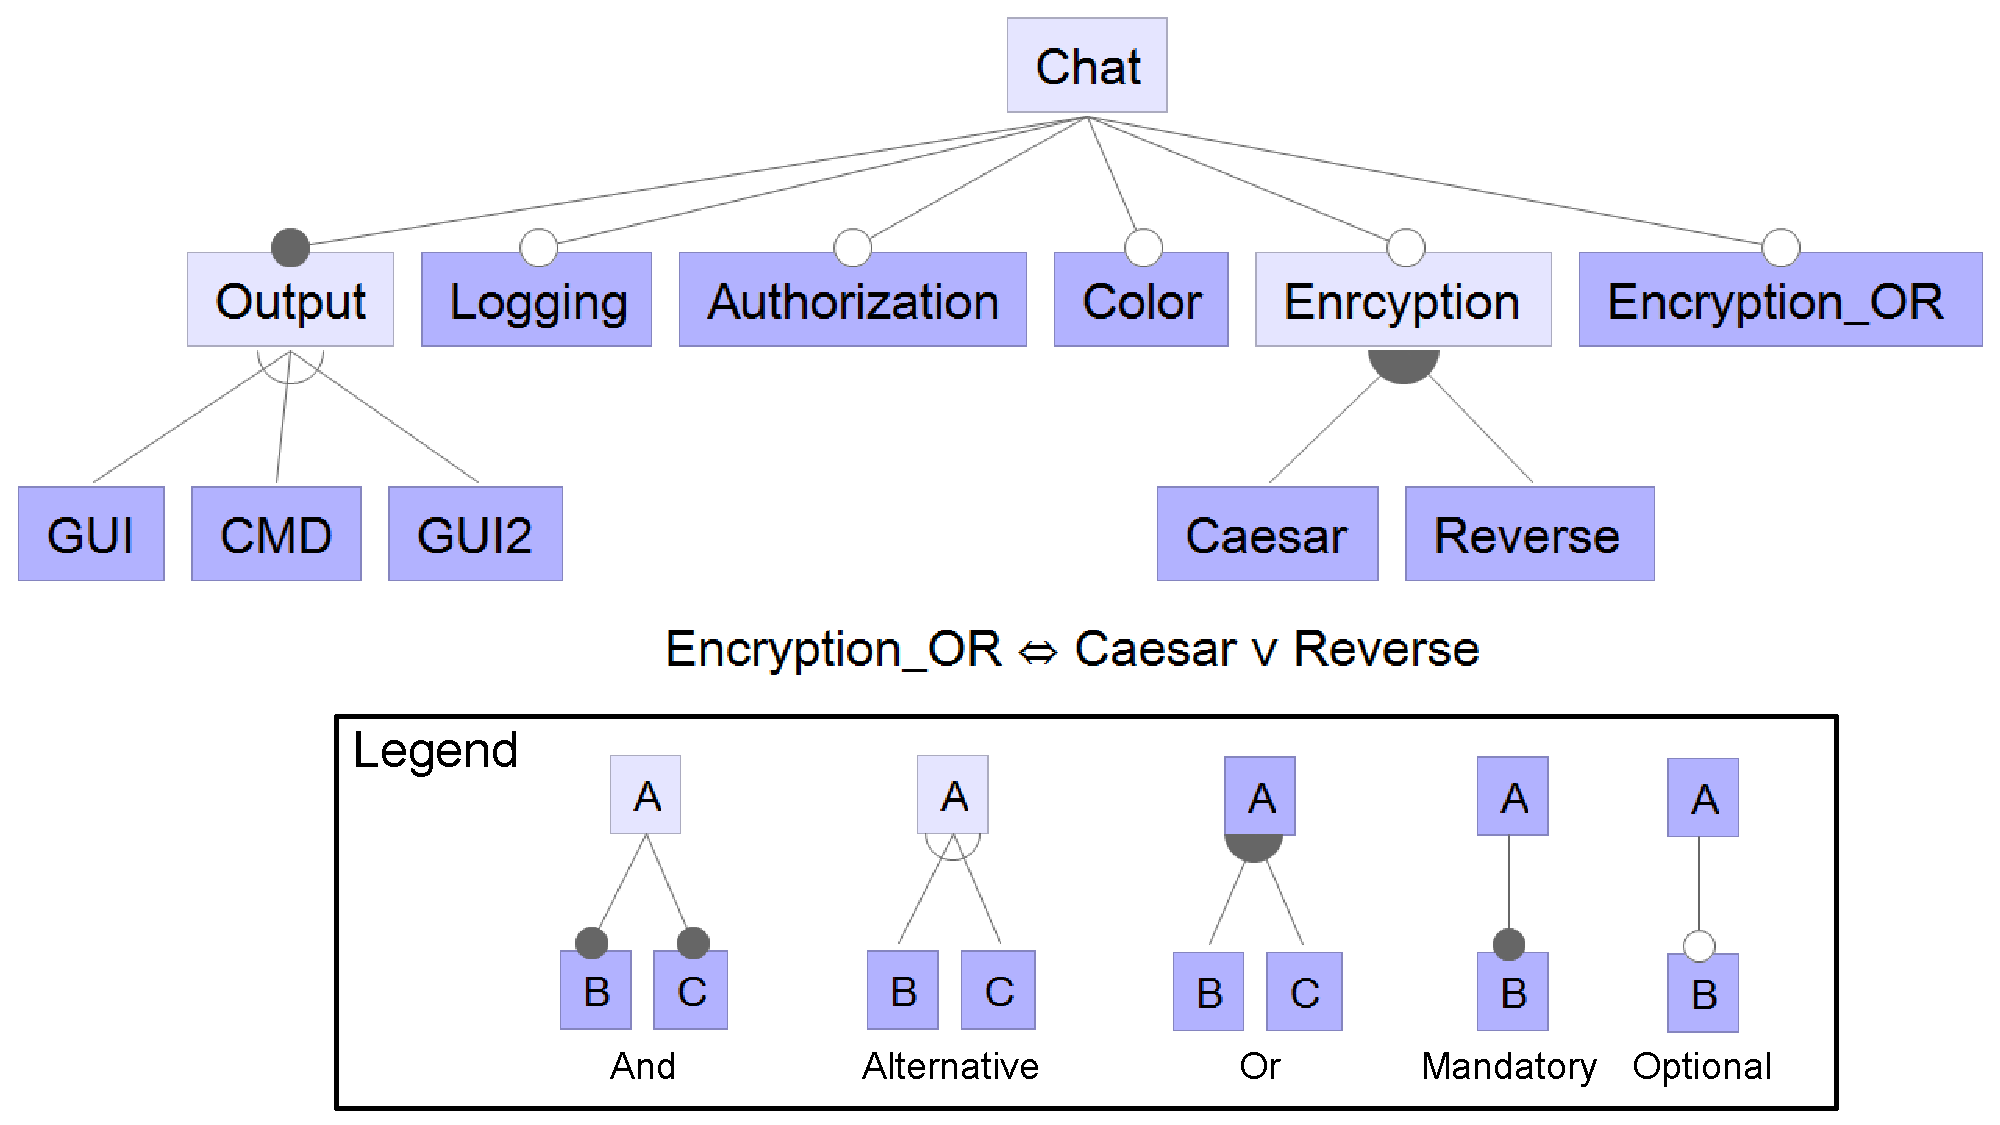
\epsfig{file=image/fm.bmp, width=8.5cm}
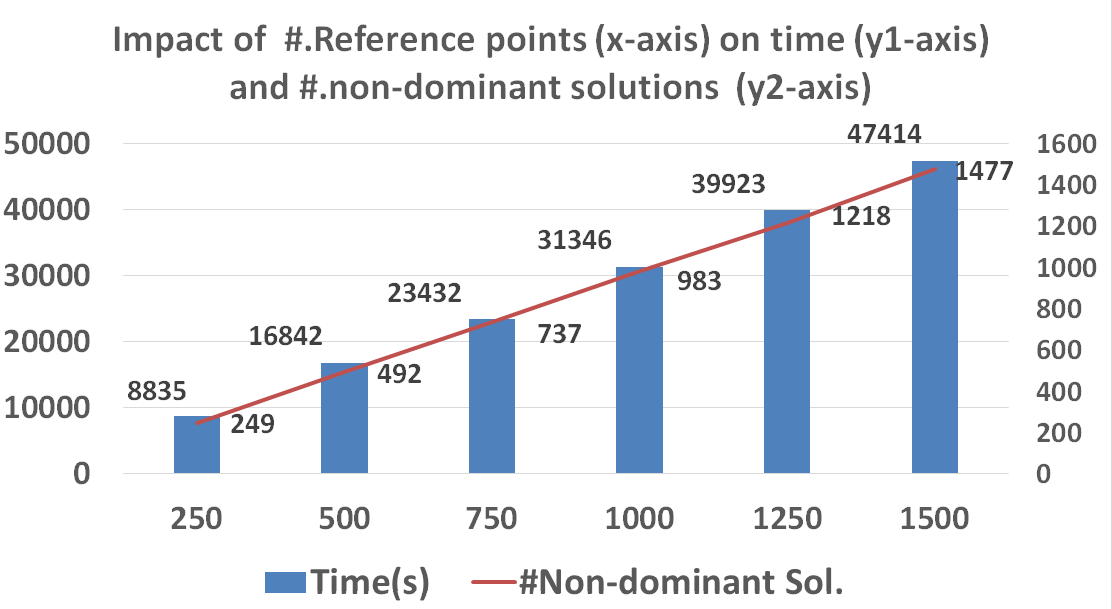
\includegraphics[width= 9cm]{image/rf.png}
\vspace{-6mm}
\caption{Impact of \#. reference points (x-axis) on execution time (y1-axis) and \#.non-dominant solutions (y2-axis) found on \emph{Linux X86 1} }
\label{fig:referPoint}
\end{figure}
